\scanpage{47}
\mspage{3)}
% archive sheet number: 46
qui forment un groupoïde \deleted{\unsure{MD}} $\unsure{\mathrm{Grbip}|\mathrm{Grabip}}$ ou $(\mathrm{Grabipond})$

\uline{Objets}: graphes \inserted{finis} $(S,\vec A,\sigma,o)$ \inserted{$+$ structures suppl.}, (pouvant avoir des sommets isolés, des boucles fermées, a fortiori plusieurs arêtes entre deux sommets, et aussi des ``\uline{arêtes libres}'' correspondant aux pts fixes de $\sigma$) $S,\vec A$ ens. finis, $\sigma:\vec A\longrightarrow\vec A$ involution, $o:\vec A\longrightarrow S$ appl. ``origine''. On se donne de plus

% slanted
\margin{\unsure{pas assez précis}, comme \unsure{donnée} -- la pondération d'une arête doit être remplacée par celle d'un \unsure{pol.\ comb.} $T_a$ avec $\unsure{\omega(T_a)\simeq\omega(a)|\omega(T_a)\simeq\omega(0)|\omega(T_a)\simeq\omega(o)}$}
\inserted{(``sommets'', ``arcs'')}

\diagram{\begin{tikzcd}[ampersand replacement=\&]
S\arrow[r,"{\deleted{\unsure{g_0}}\unsure{\gamma|g}}"] \& \mathbb N
\end{tikzcd}}
(application ``genre'' ou ``poids'')

\margin{J'ai indiqué une pondération des sommets, mais pas des arêtes}
\figure{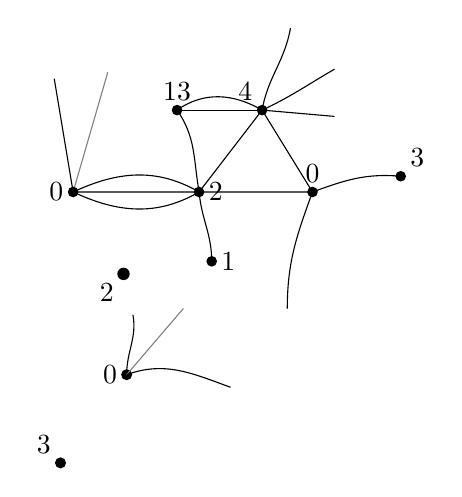
\begin{tikzpicture}[scale=.8]
\coordinate (a) at (0,2.8);\coordinate (b) at (2,2.8);\coordinate (c) at (3,4.1);\coordinate (d) at (1.65,4.1);\coordinate (e) at (3.8,2.8);\coordinate (f) at (5.2,3.05);\coordinate (g) at (2.2,1.7);
\draw (a)--(b)--(c)--(e)--(b);\draw (e) to[out=20,in=175] (f);\draw (b) to[out=-85,in=90] (g);\draw (d) to[out=-55,in=100] (b);\draw (d)--(c);\draw (d) to[out=35,in=150] (c);\draw (a) to[out=25,in=150] (b);\draw (a) to[out=-25,in=-150] (b);\draw (a) to[out=-120,in=260,looseness=6] (a);
\draw (a)--(-.3,4.6);\draw[gray] (a)--(.55,4.7);\draw (c) to[out=80,in=-100] (3.45,5.4);\draw (c) to[out=25,in=210] (4.15,4.75);\draw (c)--(4.15,4);\draw (e) to[out=-110,in=90] (3.4,.95);
\foreach \p in {a,b,c,d,e,f,g}{\fill (\p) circle (2.4pt);}
\node[left] at (a){$0$};\node[right] at (b){$2$};\node[above left] at (c){$4$};\node[above] at (d){$13$};\node[above] at (e){$0$};\node[above right] at (f){$3$};\node[right] at (g){$1$};
\fill (.8,1.5) circle (2.8pt);\node[below left] at (.8,1.5){$2$};
\fill (.85,-.1) circle (2.5pt);\node[left] at (.85,-.1){$0$};\draw (.85,-.1) to[out=90,in=-80] (.95,.85);\draw[gray] (.85,-.1)--(1.75,.95);\draw (.85,-.1) to[out=20,in=160] (2.5,-.3);
\fill (-.2,-1.5) circle (2.5pt);\node[above left] at (-.2,-1.5){$3$};\draw (-.2,-1.5) to[out=25,in=-25,looseness=7] (-.2,-1.5);
\end{tikzpicture}}

\diagram{\begin{tikzcd}[ampersand replacement=\&]
{\deleted{\unsure{\widetilde A}}\inserted{A_\ell}}\arrow[r,"{\inserted{r}\deleted{\unsure{\rho}}\unsure{r|2}}"] \& \mathbb N
\end{tikzcd}}
(application \deleted{\unsure{``multiplicité''}} ``indice de rigidification'')
\[
\deleted{\unsure{\widetilde A}\mathrel{\mathop{=}\limits^{\mathrm{def}}}\vec A/\sigma}
\]
\deleted{``\unsure{ens.\ des sommets apparents}''}

\deleted{Ou encore, posant $\widetilde S=S\amalg A_\ell$, (identif. à l'ens. de tous les ``sommets'' \inserted{apparents}, \deleted{\unsure{immergés}} et \inserted{``immergés'' (i.e. $\in S$)} les ``libres'', \inserted{\unsure{un correspondant à un $a\in A_\ell$}} du graphe), on donne}
\diagram{\begin{tikzcd}[ampersand replacement=\&]
\deleted{\widetilde S}\arrow[r,"\deleted{\pi}"] \& \deleted{\mathbb N}
\end{tikzcd}}
\deleted{(\uline{pondération} du graphe)}

\margin{$\widetilde S=S\amalg\deleted{\unsure{\widetilde S_\ell}}\inserted{A_\ell}$ \deleted{\unsure{sommets libres}}\par $\widetilde A=\vec A/\sigma=A\amalg A_\ell$}
\diagram{\begin{tikzcd}[ampersand replacement=\&]
\vec A\arrow[d]\& {=\vec A_0}\arrow[d,"\deg 2"]\arrow[d,phantom,shift left=5ex,"{\underbrace{\vec A\setminus\vec A^\sigma}}" description]\& {\amalg\vec A_\ell}\arrow[d,"\deg 1"]\arrow[d,phantom,shift left=5ex,"{\underbrace{\vec A^\sigma}}" description]\\
\widetilde A\& {=A}\& {\amalg A_\ell}
\end{tikzcd}}
\margin{Ordre d'un sommet\par $\sigma(s)=\underbrace{\sigma_\ell(s)}+\sigma_0(s)$\par \unsure{correspond} aux ``trous'' ou cercles de \unsure{recollage}}

La donnée du \uline{graphe} sous-jacent à un graphe \deleted{\unsure{MD}}\inserted{bip.} revient à celle d'un graphe ``ordinaire'' \unsure{accompagnant} (sans arêtes libres, i.e. $\sigma$ opère sans pts fixes), i.e.
\[
(S,(\vec A\setminus\vec A^\sigma),\sigma|_{(\vec A\setminus\vec A^\sigma)},o|_{\vec A\setminus\vec A^\sigma}),
\]
\uline{plus} un ensemble \inserted{fini} $A_\ell$ (\deleted{\unsure{``sommets''}}\inserted{arêtes} libres) \deleted{ou ``sommets-trous''} et une application
\diagram{\begin{tikzcd}[ampersand replacement=\&]
A_\ell\arrow[r] \& S
\end{tikzcd}}

\uline{Flèches} Les iso. de telles structures
